\documentclass[]{report}


% Title Page
\title{Title of the Homework}
\author{Burak ER}

\usepackage{psfrag}

\usepackage{amsmath}

\usepackage{amssymb}

\usepackage{pstricks, pst-node, pst-plot, pst-circ}

\usepackage{moredefs}

\usepackage{hyperref}

\usepackage{cleveref}

\usepackage{graphicx}

\usepackage{epstopdf}

\usepackage{epsfig}

\usepackage{algorithm}

\usepackage{program}

\usepackage{graphicx}

\usepackage{caption}

\usepackage{subcaption}

\usepackage[autolinebreaks,useliterate]{mcode}

\crefname{lstlisting}{listing}{listings}

\Crefname{lstlisting}{Listing}{Listings}

\begin{document}


\maketitle
\begin{abstract}
Includes the solutions for the $number$th homework problems of \emph{A Hard} class given at Bursa Technical University, in $...$ semester year $20..$.
\\
\\
Written using \LaTeX ...
\end{abstract}
\section*{Problem 1}
Sızıntı (spektral leakage)

An equation..
\begin{align*}
\mathbf{M}=\left[\begin{array}{cccc}
m&0&0&0\\
0&I_x&0&0 \\
0&0&m_1&0 \\
0&0&0&m_2
\end{array}\right]
\end{align*}

\subsection*{Subquestion}

\begin{enumerate}
\item Find this and this...
\begin{enumerate}
\item Using this...
\item Use that... 
\end{enumerate}
\item Find the ...
\end{enumerate}

\begin{center}
\subsection*{Solution 1}
\end{center}
\textbf{Find this and this...}\\~\\
Here goes the solution...
A numbered equation...
\begin{align}
\mathrm{det}\left(-\lambda^2\mathbf{M}+ \mathbf{K}\right)=0
\label{equ:myuselessequation}
\end{align}
Using the equation \cref{equ:myuselessequation}, it is found that ...\\~\\
In \cref{fig:timedependenttires}, it is given that ...
\begin{figure}[ht!]
\centering
% This file is generated by the MATLAB m-file laprint.m. It can be included
% into LaTeX documents using the packages graphicx, color and psfrag.
% It is accompanied by a postscript file. A sample LaTeX file is:
%    \documentclass{article}\usepackage{graphicx,color,psfrag}
%    \begin{document}% This file is generated by the MATLAB m-file laprint.m. It can be included
% into LaTeX documents using the packages graphicx, color and psfrag.
% It is accompanied by a postscript file. A sample LaTeX file is:
%    \documentclass{article}\usepackage{graphicx,color,psfrag}
%    \begin{document}% This file is generated by the MATLAB m-file laprint.m. It can be included
% into LaTeX documents using the packages graphicx, color and psfrag.
% It is accompanied by a postscript file. A sample LaTeX file is:
%    \documentclass{article}\usepackage{graphicx,color,psfrag}
%    \begin{document}\input{allmode}\end{document}
% See http://www.mathworks.de/matlabcentral/fileexchange/loadFile.do?objectId=4638
% for recent versions of laprint.m.
%
% created by:           LaPrint version 3.16 (13.9.2004)
% created on:           05-Jan-2014 21:04:15
% eps bounding box:     15 cm x 8.8506 cm
% comment:              
%
\begin{psfrags}%
\psfragscanon%
%
% text strings:
\psfrag{s01}[b][b]{\color[rgb]{0,0,0}\setlength{\tabcolsep}{0pt}\begin{tabular}{c}mode 1\\62.964 rad/sn\end{tabular}}%
\psfrag{s02}[b][b]{\color[rgb]{0,0,0}\setlength{\tabcolsep}{0pt}\begin{tabular}{c}relative displacement\end{tabular}}%
\psfrag{s05}[b][b]{\color[rgb]{0,0,0}\setlength{\tabcolsep}{0pt}\begin{tabular}{c}mode 3\\6.749[rad/sn]\end{tabular}}%
\psfrag{s07}[b][b]{\color[rgb]{0,0,0}\setlength{\tabcolsep}{0pt}\begin{tabular}{c}relative displacement\end{tabular}}%
\psfrag{s09}[b][b]{\color[rgb]{0,0,0}\setlength{\tabcolsep}{0pt}\begin{tabular}{c}mode 4\\6.517[rad/sn]\end{tabular}}%
\psfrag{s11}[b][b]{\color[rgb]{0,0,0}\setlength{\tabcolsep}{0pt}\begin{tabular}{c}relative displacement\end{tabular}}%
\psfrag{s13}[b][b]{\color[rgb]{0,0,0}\setlength{\tabcolsep}{0pt}\begin{tabular}{c}mode 2\\62.951[rad/sn]\end{tabular}}%
\psfrag{s15}[b][b]{\color[rgb]{0,0,0}\setlength{\tabcolsep}{0pt}\begin{tabular}{c}relative displacement\end{tabular}}%
%
% xticklabels:
\psfrag{x01}[t][t]{0}%
\psfrag{x02}[t][t]{0.1}%
\psfrag{x03}[t][t]{0.2}%
\psfrag{x04}[t][t]{0.3}%
\psfrag{x05}[t][t]{0.4}%
\psfrag{x06}[t][t]{0.5}%
\psfrag{x07}[t][t]{0.6}%
\psfrag{x08}[t][t]{0.7}%
\psfrag{x09}[t][t]{0.8}%
\psfrag{x10}[t][t]{0.9}%
\psfrag{x11}[t][t]{1}%
\psfrag{x12}[t][t]{1}%
\psfrag{x13}[t][t]{1.5}%
\psfrag{x14}[t][t]{2}%
\psfrag{x15}[t][t]{2.5}%
\psfrag{x16}[t][t]{3}%
\psfrag{x17}[t][t]{3.5}%
\psfrag{x18}[t][t]{4}%
\psfrag{x19}[t][t]{1}%
\psfrag{x20}[t][t]{2}%
\psfrag{x21}[t][t]{3}%
\psfrag{x22}[t][t]{4}%
\psfrag{x23}[t][t]{1}%
\psfrag{x24}[t][t]{2}%
\psfrag{x25}[t][t]{3}%
\psfrag{x26}[t][t]{4}%
\psfrag{x27}[t][t]{1}%
\psfrag{x28}[t][t]{2}%
\psfrag{x29}[t][t]{3}%
\psfrag{x30}[t][t]{4}%
%
% yticklabels:
\psfrag{v01}[r][r]{0}%
\psfrag{v02}[r][r]{0.1}%
\psfrag{v03}[r][r]{0.2}%
\psfrag{v04}[r][r]{0.3}%
\psfrag{v05}[r][r]{0.4}%
\psfrag{v06}[r][r]{0.5}%
\psfrag{v07}[r][r]{0.6}%
\psfrag{v08}[r][r]{0.7}%
\psfrag{v09}[r][r]{0.8}%
\psfrag{v10}[r][r]{0.9}%
\psfrag{v11}[r][r]{1}%
\psfrag{v12}[r][r]{-1}%
\psfrag{v13}[r][r]{-0.5}%
\psfrag{v14}[r][r]{0}%
\psfrag{v15}[r][r]{0.5}%
\psfrag{v16}[r][r]{1}%
\psfrag{v17}[r][r]{-1}%
\psfrag{v18}[r][r]{-0.5}%
\psfrag{v19}[r][r]{0}%
\psfrag{v20}[r][r]{0.5}%
\psfrag{v21}[r][r]{1}%
\psfrag{v22}[r][r]{-1}%
\psfrag{v23}[r][r]{-0.5}%
\psfrag{v24}[r][r]{0}%
\psfrag{v25}[r][r]{0.5}%
\psfrag{v26}[r][r]{1}%
\psfrag{v27}[r][r]{-1}%
\psfrag{v28}[r][r]{-0.5}%
\psfrag{v29}[r][r]{0}%
\psfrag{v30}[r][r]{0.5}%
\psfrag{v31}[r][r]{1}%
%
% Figure:
\resizebox{10cm}{!}{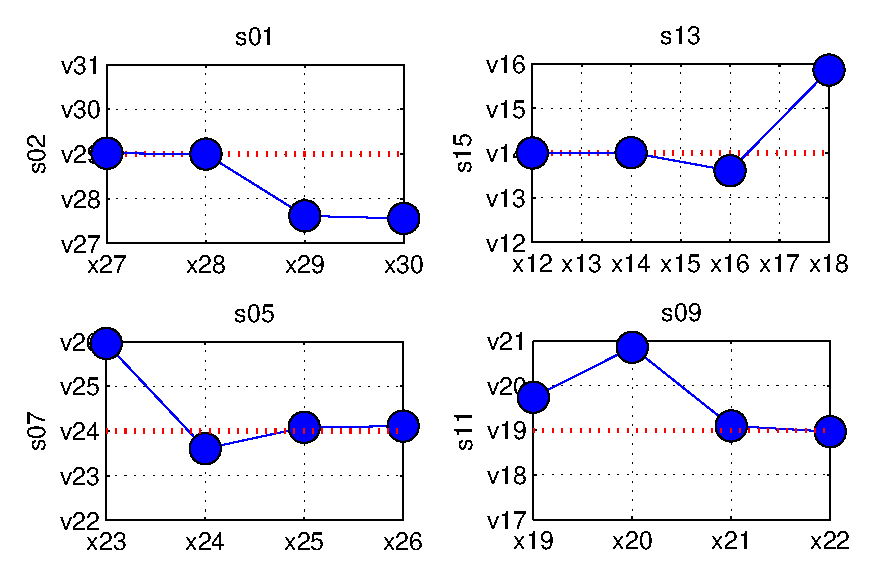
\includegraphics{./Figures/allmode.eps}}%
\end{psfrags}%
%
% End allmode.tex
\end{document}
% See http://www.mathworks.de/matlabcentral/fileexchange/loadFile.do?objectId=4638
% for recent versions of laprint.m.
%
% created by:           LaPrint version 3.16 (13.9.2004)
% created on:           05-Jan-2014 21:04:15
% eps bounding box:     15 cm x 8.8506 cm
% comment:              
%
\begin{psfrags}%
\psfragscanon%
%
% text strings:
\psfrag{s01}[b][b]{\color[rgb]{0,0,0}\setlength{\tabcolsep}{0pt}\begin{tabular}{c}mode 1\\62.964 rad/sn\end{tabular}}%
\psfrag{s02}[b][b]{\color[rgb]{0,0,0}\setlength{\tabcolsep}{0pt}\begin{tabular}{c}relative displacement\end{tabular}}%
\psfrag{s05}[b][b]{\color[rgb]{0,0,0}\setlength{\tabcolsep}{0pt}\begin{tabular}{c}mode 3\\6.749[rad/sn]\end{tabular}}%
\psfrag{s07}[b][b]{\color[rgb]{0,0,0}\setlength{\tabcolsep}{0pt}\begin{tabular}{c}relative displacement\end{tabular}}%
\psfrag{s09}[b][b]{\color[rgb]{0,0,0}\setlength{\tabcolsep}{0pt}\begin{tabular}{c}mode 4\\6.517[rad/sn]\end{tabular}}%
\psfrag{s11}[b][b]{\color[rgb]{0,0,0}\setlength{\tabcolsep}{0pt}\begin{tabular}{c}relative displacement\end{tabular}}%
\psfrag{s13}[b][b]{\color[rgb]{0,0,0}\setlength{\tabcolsep}{0pt}\begin{tabular}{c}mode 2\\62.951[rad/sn]\end{tabular}}%
\psfrag{s15}[b][b]{\color[rgb]{0,0,0}\setlength{\tabcolsep}{0pt}\begin{tabular}{c}relative displacement\end{tabular}}%
%
% xticklabels:
\psfrag{x01}[t][t]{0}%
\psfrag{x02}[t][t]{0.1}%
\psfrag{x03}[t][t]{0.2}%
\psfrag{x04}[t][t]{0.3}%
\psfrag{x05}[t][t]{0.4}%
\psfrag{x06}[t][t]{0.5}%
\psfrag{x07}[t][t]{0.6}%
\psfrag{x08}[t][t]{0.7}%
\psfrag{x09}[t][t]{0.8}%
\psfrag{x10}[t][t]{0.9}%
\psfrag{x11}[t][t]{1}%
\psfrag{x12}[t][t]{1}%
\psfrag{x13}[t][t]{1.5}%
\psfrag{x14}[t][t]{2}%
\psfrag{x15}[t][t]{2.5}%
\psfrag{x16}[t][t]{3}%
\psfrag{x17}[t][t]{3.5}%
\psfrag{x18}[t][t]{4}%
\psfrag{x19}[t][t]{1}%
\psfrag{x20}[t][t]{2}%
\psfrag{x21}[t][t]{3}%
\psfrag{x22}[t][t]{4}%
\psfrag{x23}[t][t]{1}%
\psfrag{x24}[t][t]{2}%
\psfrag{x25}[t][t]{3}%
\psfrag{x26}[t][t]{4}%
\psfrag{x27}[t][t]{1}%
\psfrag{x28}[t][t]{2}%
\psfrag{x29}[t][t]{3}%
\psfrag{x30}[t][t]{4}%
%
% yticklabels:
\psfrag{v01}[r][r]{0}%
\psfrag{v02}[r][r]{0.1}%
\psfrag{v03}[r][r]{0.2}%
\psfrag{v04}[r][r]{0.3}%
\psfrag{v05}[r][r]{0.4}%
\psfrag{v06}[r][r]{0.5}%
\psfrag{v07}[r][r]{0.6}%
\psfrag{v08}[r][r]{0.7}%
\psfrag{v09}[r][r]{0.8}%
\psfrag{v10}[r][r]{0.9}%
\psfrag{v11}[r][r]{1}%
\psfrag{v12}[r][r]{-1}%
\psfrag{v13}[r][r]{-0.5}%
\psfrag{v14}[r][r]{0}%
\psfrag{v15}[r][r]{0.5}%
\psfrag{v16}[r][r]{1}%
\psfrag{v17}[r][r]{-1}%
\psfrag{v18}[r][r]{-0.5}%
\psfrag{v19}[r][r]{0}%
\psfrag{v20}[r][r]{0.5}%
\psfrag{v21}[r][r]{1}%
\psfrag{v22}[r][r]{-1}%
\psfrag{v23}[r][r]{-0.5}%
\psfrag{v24}[r][r]{0}%
\psfrag{v25}[r][r]{0.5}%
\psfrag{v26}[r][r]{1}%
\psfrag{v27}[r][r]{-1}%
\psfrag{v28}[r][r]{-0.5}%
\psfrag{v29}[r][r]{0}%
\psfrag{v30}[r][r]{0.5}%
\psfrag{v31}[r][r]{1}%
%
% Figure:
\resizebox{10cm}{!}{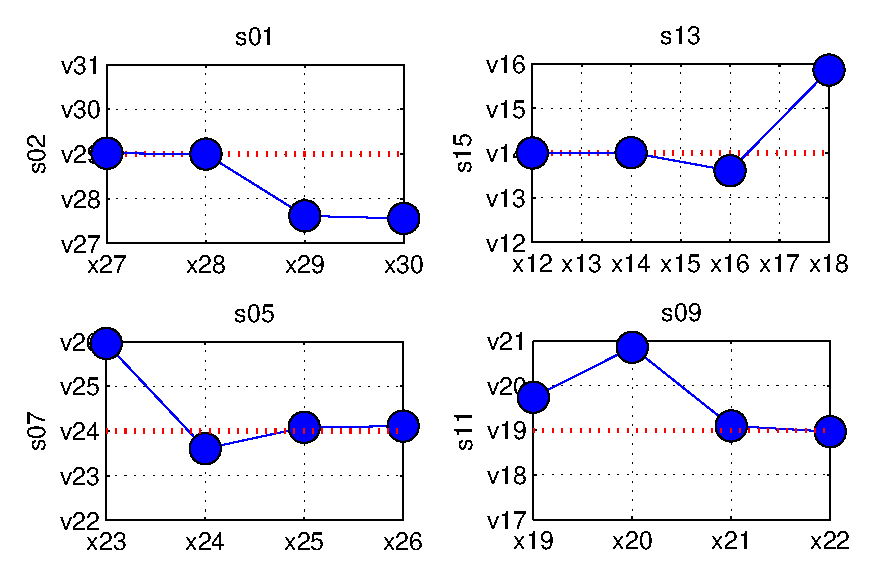
\includegraphics{./Figures/allmode.eps}}%
\end{psfrags}%
%
% End allmode.tex
\end{document}
% See http://www.mathworks.de/matlabcentral/fileexchange/loadFile.do?objectId=4638
% for recent versions of laprint.m.
%
% created by:           LaPrint version 3.16 (13.9.2004)
% created on:           05-Jan-2014 21:04:15
% eps bounding box:     15 cm x 8.8506 cm
% comment:              
%
\begin{psfrags}%
\psfragscanon%
%
% text strings:
\psfrag{s01}[b][b]{\color[rgb]{0,0,0}\setlength{\tabcolsep}{0pt}\begin{tabular}{c}mode 1\\62.964 rad/sn\end{tabular}}%
\psfrag{s02}[b][b]{\color[rgb]{0,0,0}\setlength{\tabcolsep}{0pt}\begin{tabular}{c}relative displacement\end{tabular}}%
\psfrag{s05}[b][b]{\color[rgb]{0,0,0}\setlength{\tabcolsep}{0pt}\begin{tabular}{c}mode 3\\6.749[rad/sn]\end{tabular}}%
\psfrag{s07}[b][b]{\color[rgb]{0,0,0}\setlength{\tabcolsep}{0pt}\begin{tabular}{c}relative displacement\end{tabular}}%
\psfrag{s09}[b][b]{\color[rgb]{0,0,0}\setlength{\tabcolsep}{0pt}\begin{tabular}{c}mode 4\\6.517[rad/sn]\end{tabular}}%
\psfrag{s11}[b][b]{\color[rgb]{0,0,0}\setlength{\tabcolsep}{0pt}\begin{tabular}{c}relative displacement\end{tabular}}%
\psfrag{s13}[b][b]{\color[rgb]{0,0,0}\setlength{\tabcolsep}{0pt}\begin{tabular}{c}mode 2\\62.951[rad/sn]\end{tabular}}%
\psfrag{s15}[b][b]{\color[rgb]{0,0,0}\setlength{\tabcolsep}{0pt}\begin{tabular}{c}relative displacement\end{tabular}}%
%
% xticklabels:
\psfrag{x01}[t][t]{0}%
\psfrag{x02}[t][t]{0.1}%
\psfrag{x03}[t][t]{0.2}%
\psfrag{x04}[t][t]{0.3}%
\psfrag{x05}[t][t]{0.4}%
\psfrag{x06}[t][t]{0.5}%
\psfrag{x07}[t][t]{0.6}%
\psfrag{x08}[t][t]{0.7}%
\psfrag{x09}[t][t]{0.8}%
\psfrag{x10}[t][t]{0.9}%
\psfrag{x11}[t][t]{1}%
\psfrag{x12}[t][t]{1}%
\psfrag{x13}[t][t]{1.5}%
\psfrag{x14}[t][t]{2}%
\psfrag{x15}[t][t]{2.5}%
\psfrag{x16}[t][t]{3}%
\psfrag{x17}[t][t]{3.5}%
\psfrag{x18}[t][t]{4}%
\psfrag{x19}[t][t]{1}%
\psfrag{x20}[t][t]{2}%
\psfrag{x21}[t][t]{3}%
\psfrag{x22}[t][t]{4}%
\psfrag{x23}[t][t]{1}%
\psfrag{x24}[t][t]{2}%
\psfrag{x25}[t][t]{3}%
\psfrag{x26}[t][t]{4}%
\psfrag{x27}[t][t]{1}%
\psfrag{x28}[t][t]{2}%
\psfrag{x29}[t][t]{3}%
\psfrag{x30}[t][t]{4}%
%
% yticklabels:
\psfrag{v01}[r][r]{0}%
\psfrag{v02}[r][r]{0.1}%
\psfrag{v03}[r][r]{0.2}%
\psfrag{v04}[r][r]{0.3}%
\psfrag{v05}[r][r]{0.4}%
\psfrag{v06}[r][r]{0.5}%
\psfrag{v07}[r][r]{0.6}%
\psfrag{v08}[r][r]{0.7}%
\psfrag{v09}[r][r]{0.8}%
\psfrag{v10}[r][r]{0.9}%
\psfrag{v11}[r][r]{1}%
\psfrag{v12}[r][r]{-1}%
\psfrag{v13}[r][r]{-0.5}%
\psfrag{v14}[r][r]{0}%
\psfrag{v15}[r][r]{0.5}%
\psfrag{v16}[r][r]{1}%
\psfrag{v17}[r][r]{-1}%
\psfrag{v18}[r][r]{-0.5}%
\psfrag{v19}[r][r]{0}%
\psfrag{v20}[r][r]{0.5}%
\psfrag{v21}[r][r]{1}%
\psfrag{v22}[r][r]{-1}%
\psfrag{v23}[r][r]{-0.5}%
\psfrag{v24}[r][r]{0}%
\psfrag{v25}[r][r]{0.5}%
\psfrag{v26}[r][r]{1}%
\psfrag{v27}[r][r]{-1}%
\psfrag{v28}[r][r]{-0.5}%
\psfrag{v29}[r][r]{0}%
\psfrag{v30}[r][r]{0.5}%
\psfrag{v31}[r][r]{1}%
%
% Figure:
\resizebox{10cm}{!}{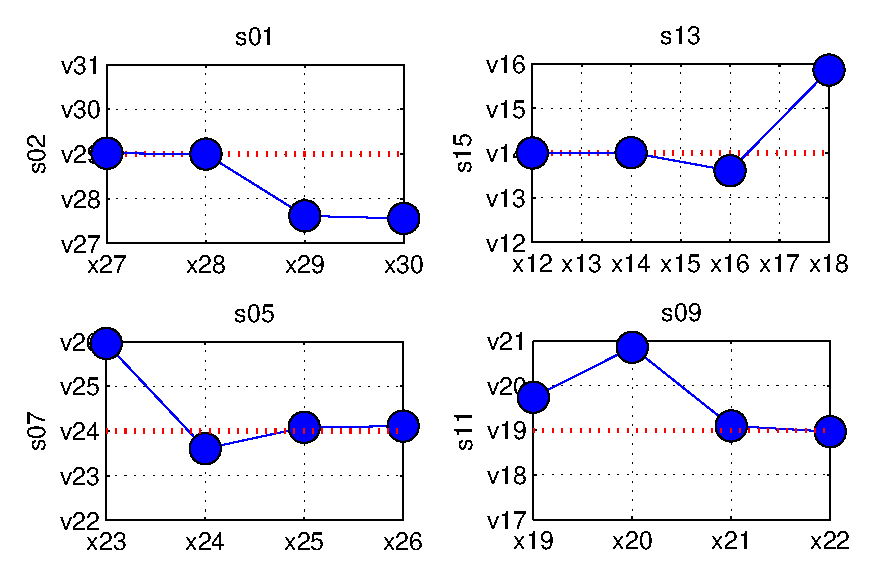
\includegraphics{./Figures/allmode.eps}}%
\end{psfrags}%
%
% End allmode.tex

\caption{A Figure that is output of LaPrint using Matlab. Use input command to include graphics.}
\label{fig:timedependenttires}
\end{figure}
\\~\\
\section*{Problem 2}
Another problem definition...
\subsection*{Question 1}
\textbf{Text of the question 1}
\begin{center}
\subsection*{Solution 1 of Problem 2}
\end{center}
An equation...
\begin{align*}
 EI~\cfrac{\partial^4 w}{\partial x^4} + \rho A~\cfrac{\partial^2 w}{\partial t^2} = 0
\end{align*}
An enumaration...\\
\begin{enumerate}
\item {my first item}
\item {my second item }
\item {my third item }
\item {my fourth item }
\end{enumerate}
\subsection*{Question 2}
\textbf{Text of the question 2.}
\begin{center}
\subsection*{Solution 2}
\end{center}
Solution to the problem 2.


\bibliographystyle{plain}
\bibliography{biblio}

\end{document}          


